% !TeX spellcheck = en-US
% !TeX encoding = utf8
% !TeX program = pdflatex
% !BIB program = bibtex
% -*- coding:utf-8 mod:LaTeX -*-
%%%%%%%%%%%%%%%%%%%%%%%%%%%%%%%%%%%%%%%%%%%%%%%%%%%%%%%%%%%%%
%       ELECO Paper Template
%%%%%%%%%%%%%%%%%%%%%%%%%%%%%%%%%%%%%%%%%%%%%%%%%%%%%%%%%%%%%
\RequirePackage{fix-cm}
% Use extarticle document class to get 9pt main text
\documentclass[9pt]{extarticle}
\usepackage{eleco}  % Must have eleco.sty available

\usepackage{graphicx}
\usepackage{hyperref}
\hypersetup{hidelinks,
  colorlinks=true,
  allcolors=black,
  pdfstartview=Fit,
  breaklinks=true}

% For column type with wrapping and centered horizontal alignment
\usepackage{array}
\newcommand{\PreserveBackslash}[1]{\let\temp=\\#1\let\\=\temp}
\newcolumntype{C}[1]{>{\PreserveBackslash\centering}p{#1}}

% For footnotes below table within the table float
\usepackage{threeparttable}

%enable \cref{...} and \Cref{...} instead of \ref: Type of reference included in the link
\usepackage[capitalise,nameinlink]{cleveref}
% The following are to comply with the IEEE style guide.
\crefformat{equation}{#2(#1)#3}
\Crefformat{equation}{#2Equation (#1)#3}
\crefname{figure}{Fig.}{Figs.}

\title{Preparation of Papers for ELECO’2023}
\name{First Author\textsuperscript{1}, Second Author\textsuperscript{2}, and Third Author\textsuperscript{1}}
\address{\textsuperscript{1}Affiliation of first author, Address, Country \\
first.author@e-mail.address, third.author@e-mail.address\\
\textsuperscript{2}Affiliation of second author, Address, Country\\
second.author@e-mail.address}

\begin{document}
\bstctlcite{IEEEexample:BSTcontrol}

\maketitle

%%%%%%%%%%%%%%
\begin{abstract}
This document gives you guidelines for preparing papers for the international conference ELECO’2023. You can use this document as a template if you are using \LaTeX. Otherwise, you can use this document as an instruction set. The papers should begin with an abstract. The abstract should not exceed 150 words. The word ``Abstract'' as the title, in 10-point Times, boldface type, centered relative to the column, initially capitalized. The abstract is to be in 9-point Times, boldface type, single-spaced type. Content of the abstract is aligned with both edges of the column.
\end{abstract}

\section{Introduction}

ELECO has been organizing as an international conference in every odd numbered year and as a national conference in every even numbered year. So, we have reached to the ELECO 2023 14th international conference with participants coming from various countries presenting papers across the broad spectrum of electrical and electronics engineering. ELECO 2023 is jointly organized by Bursa Uludag University; Istanbul Technical University (ITU); and the Chamber of Turkish Electrical Engineers (EMO), Bursa Branch.

This document is a template for Microsoft Word. You can download the electronic file of this document from \url{http://www.eleco.org.tr}. The papers should write in English.

The written material of the paper should prepare on a paper of A4 (21 cm width and 29.7 cm height) size. Five pages are allowed for each paper (including title, author(s), abstract, text, figures, tables and references).

\section{Page Arrangement}

The manuscripts must be prepared in a two-column format on A4 size paper. The margins on the first page must be as follows: top = 3 cm, bottom = 3.7 cm, left = 2 cm, right = 2 cm. All margins on the second and subsequent pages: top = 2.5 cm, bottom = 3.7 cm, left = 2 cm, right = 2 cm.

The text of the paper must be written in two columns with a space of 0.5 cm between them (Fig. 1). The width of each column must be 8.25 cm.

On the last page of the paper, the lengths of the columns must be adjusted so that they are equal. Do not add page numbers.

All the text must be written in Times New Roman fonts, single line spacing. The exception may be done for the contents of tables and figures, where Arial as well as Times New Roman font may be used. Font sizes and styles are listed in Table 1.

All paragraphs should be indented 0.4 mm. Please do not place any additional blank lines between paragraphs. Be sure your text is fully justified.

\begin{figure}[!h]
	\centering
	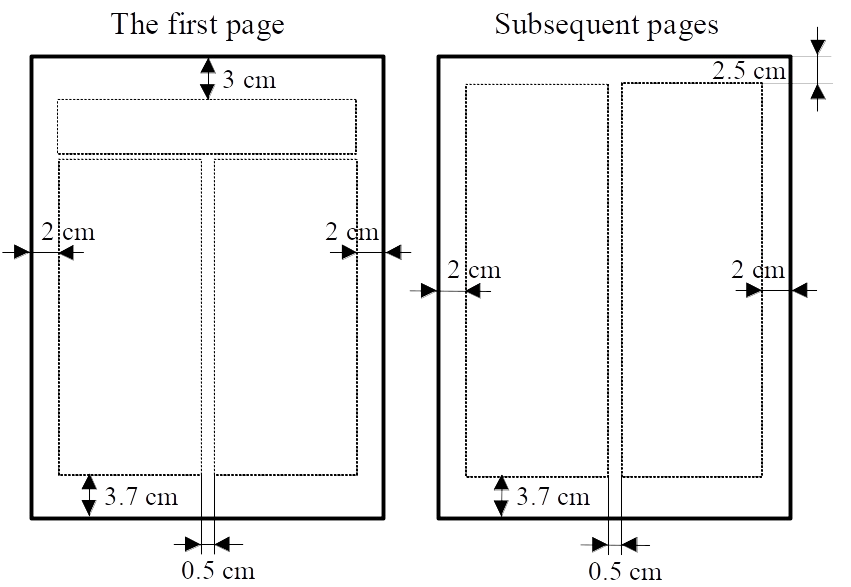
\includegraphics[width=1.0\columnwidth]{page-layout.png}
	\caption{Arrangement of printing area on an A4 size page for the first and subsequent pages of the manuscript}
	\label{fig:page-layout}
\end{figure}

\begin{table}[!h]
	\centering
	\begin{threeparttable}
	\caption{Font sizes and styles}
	\label{table:fonts}
	\setlength\tabcolsep{0.3mm}
	\begin{tabular}{|C{29.4mm}|C{12.59mm}|C{38.69mm}|}
	\hline
	  & Size & Style \\ \hline
	  Title of the Paper & 14 pt* & \textbf{Bold}, Initially capitalized \\ \hline
	  Name of Author(s) & 11 pt & Regular \\ \hline
	  Affiliation(s) & 10 pt & Regular \\ \hline
	  Text of the Abstract & 9 pt & \textbf{Bold} \\ \hline
	  Text of the Paper & 9 pt & Regular \\ \hline
	  Headings of chapters and subsections & 10 pt & \textbf{Bold}, Initially capitalized \\ \hline
	  Caption of Table & 9 pt & Regular \ (The word ``Table'' and number -- \textbf{Bold}) \\ \hline
	  Contents of Table & 9 pt & Regular \\ \hline
	  Caption of Figure & 9 pt & Regular (The word ``Fig.'' and number -- \textbf{Bold}) \\ \hline
	  Subscripts and Superscripts & 7 pt & Regular \\	
	\hline
	\end{tabular}
	\begin{tablenotes}[flushleft]
		\item * 1 point (pt) is about 0.35 mm.
	\end{tablenotes}
	\end{threeparttable}
\end{table}

\subsection{First Page}

The first page of the manuscript must contain the title of the paper, author(s) name(s) and affiliation(s) all centered on the top of the page and spanning both columns. The title should be written using 14-point Times, boldface type with single spacing. Initially capitalize nouns, pronouns, verbs, adjectives, and adverbs; do not capitalize articles, coordinate conjunctions, or prepositions (unless the title begins with such a word).

Full names of authors are preferred, but initials may be used instead. There must be one-line separations between the title and author name(s), and between the authors and their affiliation(s). A two-line separation is required between the author affiliation(s) and the start of the main text.

\subsection{Headings}

Headings of chapters should be written in 10-point bold type font with single spacing. They should be numbered by successive Arabic numerals and centered in lines. Titles of subsections are to be written in 10-point bold type font with single-spacing as well, but they should be aligned with the left edge of the column. Full-stop symbol follows the number of chapter or subsection. All titles must be separated from the text by one (9-point) blank line above, and one (9-point) blank line below the title.

\section{Figures and Tables}

Figures and tables should be not more than 8.25 cm wide and ought to be centered in column. If possible, position figures and tables at the tops and bottoms of columns. Large figures and tables (maximum 17 cm width) may span across both columns. In such cases they should be centered on the full width of page together with captions or headings.

\subsection{Figures}

Captions of figures should be aligned with both edges of the column below the figures, in 9-point font, single spacing. The word ``Fig.'' and the successive Arabic number with the full-stop symbol (``.'') must be written in bold. There should not be a full-stop symbol in the end of the caption of figure or table. Above each figure and below its caption should be 1 blank line spacing (9-point). The space between figure and its caption should have the size of approximately 6-point font.

All figures must be cited in the text in a consecutive order using abbreviations, e.g. ``\cref{fig:page-layout}''. In figure axis labels, use words rather than symbols. Put units in parentheses. For example, write ``Time (s)''. Do not label axes only with units.

\subsection{Tables}

Every table must have a descriptive title. Captions of tables should be aligned with both edges of the column above the tables, in 9-point font, single spacing. The word ``Table'' and the successive Arabic number with the full-stop symbol (``.'') must be written in bold. Below each table and above its caption should be 1 blank line spacing (9-point). The caption should be separated from the table by one 6-point empty line. Tables must be cited consecutively in the text, e.g. ``Table 1''.


\section{Equations}

Equations ought to be centrally arranged in lines and numbered by successive Arabic numerals using parentheses aligned with the right-side edge of the column. Symbols and variables in the equations as well as in the text should be written in italics, while vectors and matrices in ordinary bold type.

The equations ought to be separated from the text by 1 blank line (9-point):
%
\begin{equation}
	\label{eqn:voltage-sine}
	u(t) = U_m \cdot \sin \omega t
\end{equation}

Symbols in the equation should be defined before the equation appears or immediately following.

\section{Abbreviations and Units}

Define abbreviations and acronyms the first time they are used in the text, even if they have been defined in the abstract. Commonly used abbreviations such as IEC, IEEE, SI, AC, and RMS do not have to be defined. Use SI units where possible.

\section{Conclusions}

The instruction for the preparation of paper manuscripts for the international conference ELECO 2023 provides the essential arrangement and technical requirements for papers. This template can be downloaded from \url{http://eleco.emo.org.tr}.

The full papers should be uploaded by the corresponding author of the manuscript through web upload system on \url{http://www.eleco.org.tr}. Only online submissions are accepted to facilitate rapid publication. The submitted file should be in PDF format.

Organization committee of ELECO 2023 would like to thank you for preparation of your paper according to the instruction.

\section{References}

All references must be numbered consecutively by Arabic numerals. All references should be cited within the text using numbers in square brackets, e.g. ``\cite{journal_paper,book}''. All references must be listed in 9-point Times, single-spaced, at the end of the paper as following examples:
\nocite{*}

\bibliography{IEEEabrv,biblio}

\end{document}
